\newcommand{\ClassPath}{../../VIU_TFM_LaTeX_template}
\documentclass{\ClassPath/viu-tfm-template}
\usepackage{multicol}

\definecolor{maincolor}{HTML}{f25416}

%--------------------------------------------------------------------------
% Definiciones necesarias Modifica con tus datos
%--------------------------------------------------------------------------
\def\nombre{Gómez Olivencia, Rubén}
\def\dni{78910013-A}
\def\titulo{Prototipado y diseño de navegación \linebreak\linebreak\linebreak para la Asociación Internacional de Chefs}
\def\titulacion{Máster Universitario en Desarrollo de Aplicaciones y Servicios Web}
\def\curso{2022-2023}

%Los siguientes son opcionales: si no se ponen, la portada cambia un poco. Ideal para escribir artículos/trabajos cortos
\def\dirige{}
\def\convocatoria{}
\def\asignatura{Ingeniería Software Web}


% importar fichero de Bibliografía
%\addbibresource{Actividad_3.bib}

\begin{document}
    \graphicspath{{../../VIU_TFM_LaTeX_template/}}

    \coverpage

    \tableofcontents

\chapter{Introducción}
A lo largo de este documento se va a analizar cómo crear  los modelos concretos y cuáles han sido las decisiones tomadas para la creación de los prototipos y diseños de navegación para la aplicación web creada para la Asociación Internacional de Chefs \textbf{AIC}.

Este documento es una continuación de un documento previo en el que se explicaba el análisis y diseño de la aplicación, por lo que varias de las decisiones aquí tomadas tienen origen en dicho documento previo.


\chapter{Justificación}
Una vez realizado el análisis de requisitos del cliente, habiendo conocido las funcionalidades mínimas que requiere y habiendo obtenido los requisitos funcionales, transaccionales, de interfaz y no funcionales, es momento de comenzar con el prototipado y el diseño de navegación que tendrá finalmente la aplicación web.

\section{Prototipos}
Debemos tener claro que un \textbf{prototipo} es una representación (o simulación) del sistema que se ha planificado y que puede contener las siguientes características:

\vspace{-1em}
\begin{itemize}
    \item Interfaz de usuario.
    \item Funcionalidades de entrada y salida.
    \item Todos los usuarios deben entender lo que se muestra en el prototipo.
\end{itemize}

Las ventajas de creación de los prototipos es que al ser un paso previo a la creación de la aplicación, podemos obtener una reacción directa del cliente y sus impresiones, ya que es probable que no entienda las especificaciones de requisitos creadas en el documento anterior. Es decir, la creación de prototipos nos va a dar un \textit{feedback} del cliente de manera rápida y sencilla.

Con los prototipos, no sólo vamos a obtener una respuesta al análisis creado previamente, sino que que durante las pruebas, nos pueden aparecer comportamientos no previstos previamente y por tanto cuestiones a modificar antes de realizar la programación de la aplicación. Este punto \textbf{nos puede ahorrar mucho tiempo y complicaciones que podrían surgir en el futuro}.

Por supuesto hay que entender que existen distintos tipos de creación de prototipos y dependiendo de la cantidad de funcionalidades añadidas al mismo pueden ser más fieles al resultado final. Es por ello que a continuación se especificará el tipo de prototipo creado.


\section{Prototipo creado}

A la hora de crear el prototipo para la aplicación de la \textbf{AIC} se ha optado por las siguientes características:

\vspace{-1em}
\begin{itemize}
    \item \textbf{Fidelidad alta}: Se ha querido crear un conjunto de pantallas que le van a proporcionar a los responsables de la \textbf{AIC} un modelo dinámico que pueden utilizar para entender cómo va a ser el resultado final.

    De esta manera, podrán dar el visto bueno a distintos apartados (como pueden ser los colores, las fuentes tipográficas utilizadas, la disposición de algunos componentes) antes de comenzar con el apartado de programación.

    \item \textbf{Uso específico}: Se ha optado por la creación de un prototipo operacional que se ha ido refinando en distintas iteraciones a medida que se iban añadiendo funcionalidades requeridas por el cliente. De esta manera, y tal como se ha dicho previamente, se han encontrado comportamientos no previstos que se han mejorado de cara a que durante la etapa de desarrollo no se pierda el tiempo.

    \item \textbf{Detalle y cantidad de funcionalidades}: Teniendo en cuenta el tipo de aplicación que quiere la \textbf{AIC}, ha sido posible generar un prototipo llamado “diagonal”. Esto quiere decir que se han modelado muchas características del sistema y con gran cantidad de detalle. Esto ha sido posible gracias a que \textbf{gran parte de las funcionalidades se han modularizado y estas se han podido reutilizar} a lo largo de distintas pantallas.

    \item \textbf{Ejecutabilidad}: El prototipo creado se puede considerar que es un \textbf{prototipo interactivo} ya que responde a ciertas entradas que realiza el usuario. Bien es cierto que al no disponer de un servicio de \textit{backend}, algunas de estas respuestas siempre son las mismas (son estáticas).
\end{itemize}

Con todo ello, se ha conseguido que los responsables de la \textbf{AIC} hayan dado una retroalimentación que hasta ahora no había sido posible, que se haya tenido en cuenta esa información para mejorar el propio prototipo y que se tendrá en cuenta durante la etapa de desarrollo de la aplicación.

A modo de resumen, el prototipo creado es un \textbf{prototipo del sistema completo} en el que se pueden visualizar, y con el que se puede interactuar para ver las distintas funcionalidades que tendrá la aplicación final. De nuevo destacar que al no contar con un sistema de \textit{backend}, el registro de usuarios o de recetas no va a funcionar (no se guardan los datos), pero todo el proceso es igual al que se verá en el resultado final.

El prototipo se puede visualizar, e interactuar con él, en la siguiente  \href{https://yuki.github.io/VIU_03MASW/preview.html}{dirección web}.


\chapter{Modelos concretos}

A continuación se van a detallar los modelos concretos de las distintas funcionalidades que tiene el prototipo creado, y que posteriormente será desarrollado en la aplicación web.

En la siguiente imagen se puede ver la página principal de la aplicación:

\begin{center}
    \vspace{-10pt}
    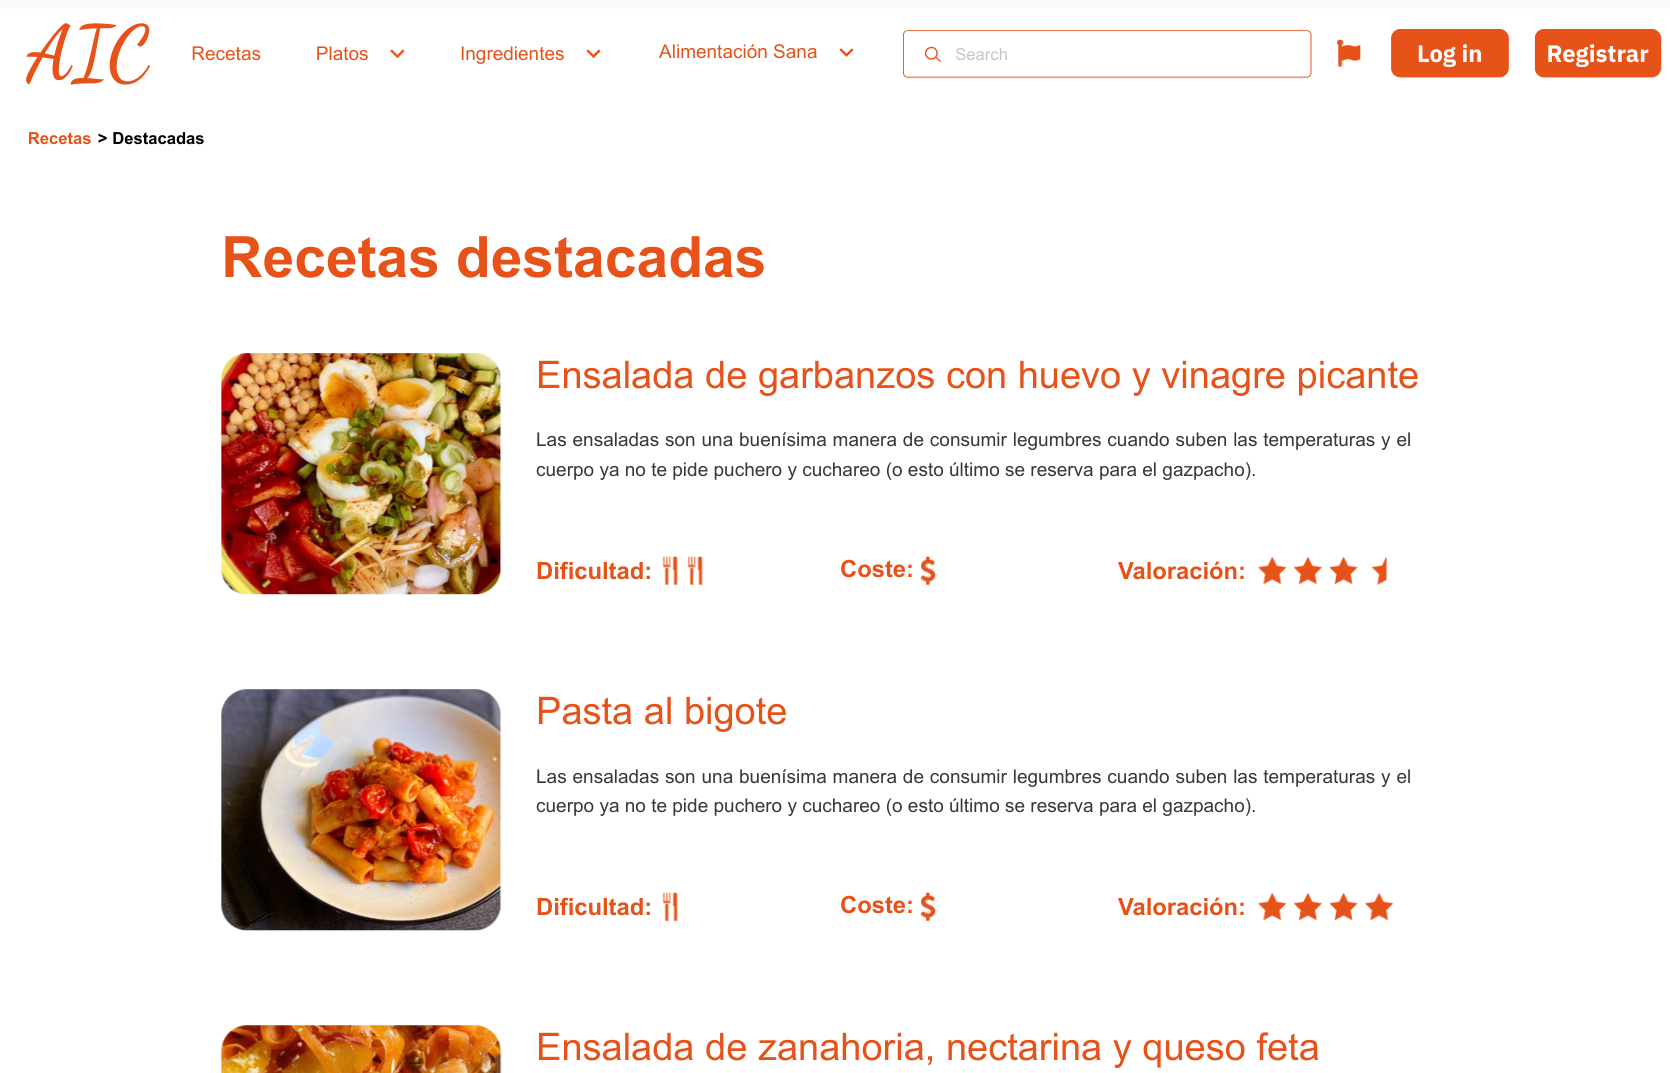
\includegraphics[frame,width=0.7\linewidth]{img/aic/0_general.png}
    \vspace{-20pt}
\end{center}

Tal como se ha dicho previamente, todo lo aquí expuesto se puede ver e interactuar a través de la siguiente \href{https://yuki.github.io/VIU_03MASW/preview.html}{dirección web}, que a su vez después también se representará a través de los esquemas de organización.

\hypertarget{menu_principal}{}
\section{Menú principal}

La aplicación web cuenta con un menú en la parte superior que es el punto de partida para que el usuario pueda acceder a distintos apartados de la aplicación. A continuación una imagen del menú:

\begin{center}
    \vspace{-10pt}
    
\includegraphics[frame,width=\linewidth]{img/aic/0_menu.png}
    \vspace{-20pt}
\end{center}

Como se puede ver, se pueden diferenciar distintas “columnas” que son secciones a las que el usuario puede acceder haciendo uso del ratón. A continuación se detallan cada una de ellas:

\vspace{-1em}
\begin{itemize}
    \item \textbf{Logotipo de AIC}: Para que se reconozca la web en la que nos encontramos, se ha añadido el logo de la \textbf{AIC}. Al hacer click sobre él se irá a la web principal de la aplicación web.
    \item \textbf{Recetas}: Es el reclamo principal del portal: la sección de recetas. Al hacer click sobre este apartado iremos a las “recetas destacadas”, que pueden ser las últimas introducidas o un aleatorio de las mismas.

    \item \textbf{Platos}: Es un menú desplegable con las categorías de los distintos tipos de platos que existen diferenciados en la aplicación. Al hacer click se despliega el menú en el que se podrá elegir la categoría que interese al usuario. Al elegir uno, se irá a un listado de recetas de dicha categoría.

    \item \textbf{Ingredientes}: Igual que el caso anterior, pero con los ingredientes. Un desplegable en el que aparecen categorizadas por familias los ingredientes que pueden ser seleccionados. Al elegir una familia de ingredientes se irá a un listado de recetas que contiene dicha familia de ingredientes.

    \item \textbf{Alimentación sana}: Es un menú en el que se puede seleccionar la nueva información que la \textbf{AIC} ha querido incorporar en la aplicación acerca de la alimentación sana.

    \item \textbf{Caja de búsqueda}: Es un cajón de búsqueda en el que el usuario podrá introducir nombre de recetas, ingredientes, tipos de platos o palabra que puede contener una receta. Al introducir las palabras y darle a la tecla “intro” se irá a la web de resultados.

    \item \textbf{Selección de idioma}: Mediante el uso del icono de una bandera, se puede modificar el idioma en el que se encuentra el portal web.

    \item \textbf{Botón de “\textit{login}”}: Para realizar la autenticación de un usuario ya registrado con su usuario y contraseña.

    \item \textbf{Botón de “registrar”}: Para aquellos usuarios que quieran introducir recetas nuevas, deben registrarse previamente a través de este botón.
    \vspace{-1em}
\end{itemize}

Es importante destacar que cuando un usuario se ha autenticado en la plataforma el menú cambia apareciendo en lugar de los botones de “Log in” y “Registrar” el menú contextual del usuario.

Todas estas secciones serán explicadas de manera detallada en las siguientes secciones y en el mapa de navegación.

\section{Camino recorrido por el usuario}

Debajo del menú, y con intención de que el usuario sepa en todo momento dónde se encuentra, aparece el “camino recorrido” de la situación actual.

\begin{center}
    \vspace{-10pt}
    \textbf{\color{maincolor}Alimentación sana > \space Ingredientes \color{black} >\space Frutos secos}
    \vspace{-15pt}
\end{center}

Teniendo en cuenta el uso de colores, también se identifican que las dos primeras palabras son enlaces que llevará al usuario a dichas secciones, mientras que el último apartado (en color negro), es el sitio actual donde se encuentra el usuario.


\section{Registro de usuario}
Continuando con lo dicho previamente, y tal como aparecen en los requisitos funcionales del documento anterior, para que un usuario pueda registrar una receta debe estar registrado en el sistema. Para que un usuario se pueda registrar debe hacer click sobre el botón “Registrar” del menú y acto seguido le aparecerá la siguiente pantalla:

\begin{center}
    \vspace{-10pt}
    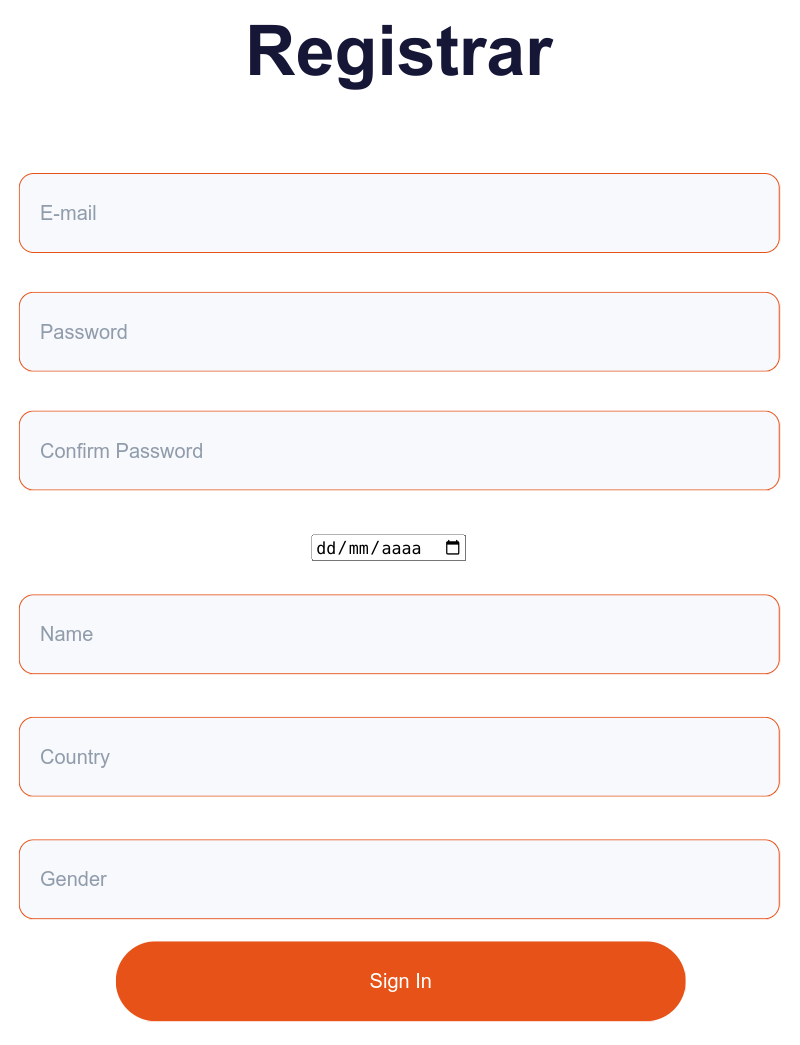
\includegraphics[frame,width=0.4\linewidth]{img/aic/registro.png}
    \vspace{-20pt}
\end{center}

Al llegar a esta pantalla, se deberán rellenar los datos y pulsar el botón para que posteriormente el usuario esté registrado en la aplicación y a partir de ahí se puedan registrar recetas.


\section{Autenticación de usuario}
Una vez el usuario ya esté registrado. Si no aparece como “logueado”, el usuario deberá darle al botón de “Log in” del menú para poder autenticarse en la aplicación. Al dar a dicho botón le aparecerá la siguiente pantalla:

\begin{center}
    \vspace{-10pt}
    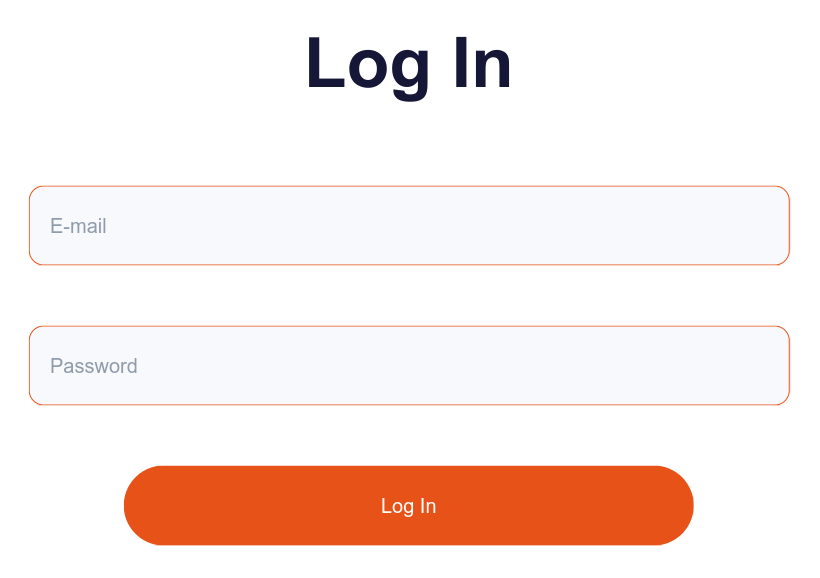
\includegraphics[frame,width=0.4\linewidth]{img/aic/login.png}
    \vspace{-20pt}
\end{center}

El usuario deberá introducir el \textit{e-mail} con el que se registró y la contraseña utilizada.

Cuando un usuario se ha autenticado, el menú principal de la aplicación cambia, desapareciendo los botones de autenticación y registro para que en su lugar aparezca lo siguiente:


\begin{center}
    \vspace{-10pt}
    
\includegraphics[frame,width=0.3\linewidth]{img/aic/logueado.png}
    \vspace{-20pt}
\end{center}

En este caso lo que aparece es el nombre del usuario, que a su vez es un desplegable, y un enlace para registrar nuevas recetas. El menú del usuario cuenta con:


\begin{multicols}{2}
    \begin{center}
        \vspace{-10pt}
        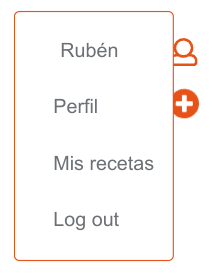
\includegraphics[width=0.8\linewidth]{img/aic/logueado_menu.png}
        \vspace{-20pt}
    \end{center}

   \begin{itemize}
       \item \textbf{Nombre de usuario}: El nombre del usuario autenticado.
       \item \textbf{Perfil}: Página donde podrá modificar su contraseña, nombre, e-mail, ...
       \item \textbf{Mis recetas}: Página donde podrá ver las recetas que ha registrado.
       \item \textbf{Log out}: Opción para dejar de estar autenticado en la plataforma.
   \end{itemize}
\end{multicols}

Todas estas opciones, como ya se ha dicho, sólo aparecen cuando el usuario está autenticado.


\section{Registrar nueva receta}

Cuando un usuario quiere registrar una nueva receta, primero debe estar autenticado como hemos visto en el punto anterior. Al hacer click sobre “{\color{maincolor}Nueva Receta}” aparecerá una nueva página donde se podrá registrar una nueva receta.

A la hora de registrar una nueva receta, habrá que rellenar distintos apartados tal como aparecen en las imágenes siguientes:


    \begin{center}
        \vspace{-10pt}
        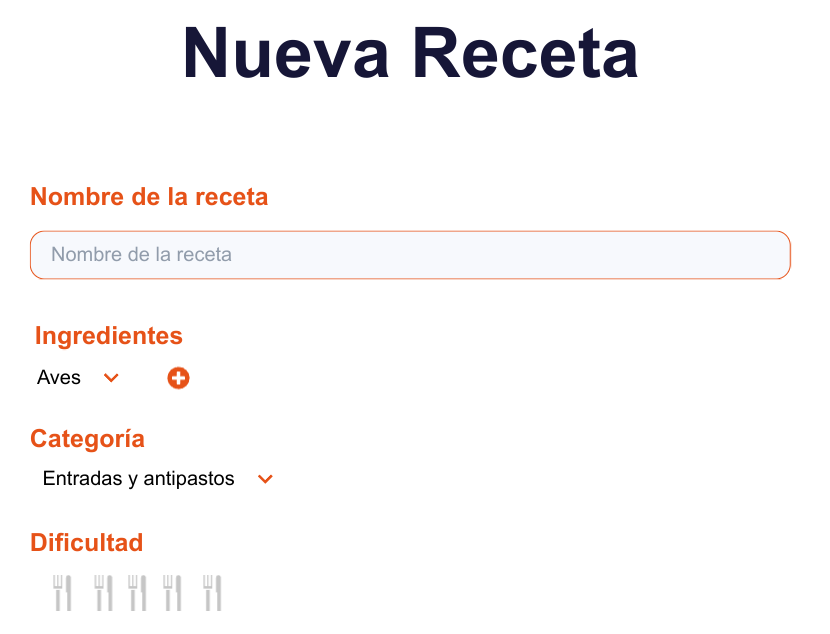
\includegraphics[width=0.6\linewidth]{img/aic/nueva_receta_1.png}
        \vspace{-20pt}
    \end{center}

    \begin{center}
        \vspace{-10pt}
        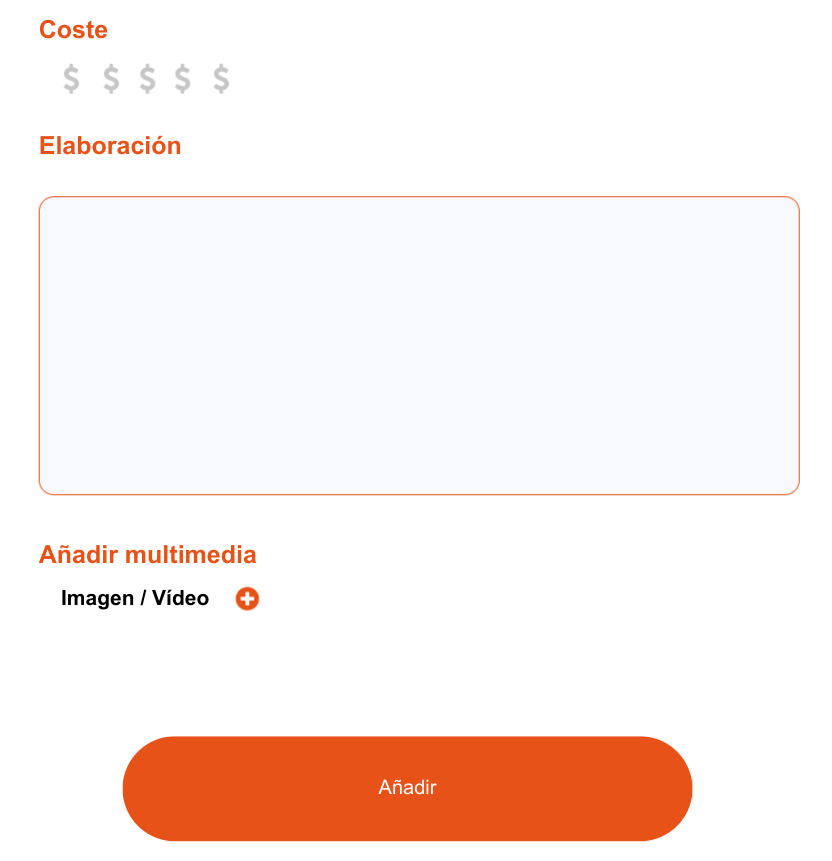
\includegraphics[width=0.6\linewidth]{img/aic/nueva_receta_2.png}
        \vspace{-20pt}
    \end{center}

Los apartados son:

\vspace{-1em}
\begin{itemize}
    \item \textbf{Nombre de la receta}: Un nombre que identifique la receta.
    \item \textbf{Ingredientes}: Es un menú desplegable junto con un icono de “+” que permitirá añadir tantos ingredientes como tenga la receta.
    \item \textbf{Categoría}: Es un menú desplegable para elegir una única categoría del plato de los requisitos indicados en el documento anterior.
    \item \textbf{Dificultad}: Para indicar la dificultad se ha optado por el uso de iconos con forma de tenedor y cuchillo, sobre los que habrá que hacer click. Indica de 1 a 5 la dificultad (de menor a mayor dificultad).
    \item \textbf{Coste}: Similar al caso anterior, pero con el símbolo de dolar para indicar el coste.
    \item \textbf{Elaboración}: Campo de texto donde el usuario podrá explicar cómo se realiza la receta.
    \item \textbf{Añadir multimedia}: Para poder añadir imágenes o vídeos de  la elaboración de la receta, se ha añadido dicha opción junto con el icono “+” para poder añadir varios ficheros.
    \item \textbf{Botón Añadir}: Una vez rellenado todos los campos, se debe pulsar el botón añadir.
\end{itemize}


\section{Búsqueda de recetas}

Una de las funcionalidades que desde la \textbf{AIC} se pedía era la posibilidad de realizar búsquedas de recetas dentro de la aplicación. Tal como se ha visto en el menú, tenemos la caja de búsqueda que permite realizar la búsqueda mediante palabras que deberán existir en la receta.

Al realizar una primera búsqueda el sistema nos permitirá realizar búsquedas ampliadas teniendo en cuenta el siguiente recuadro:

    \begin{center}
        \vspace{-10pt}
        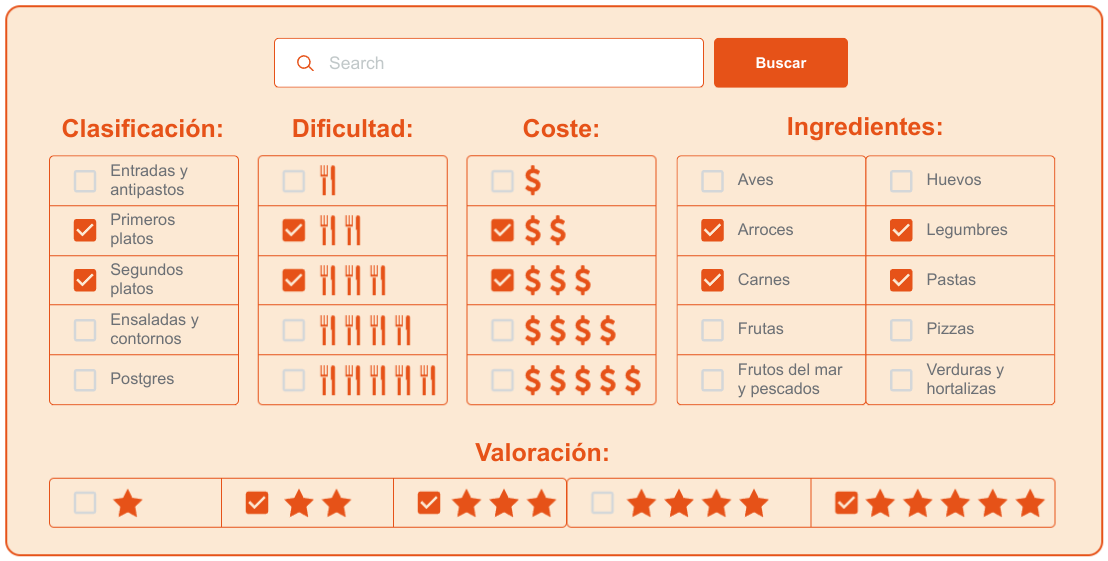
\includegraphics[width=0.8\linewidth]{img/aic/buscar.png}
        \vspace{-20pt}
    \end{center}

Como se aprecia en la imagen, este recuadro que aparecerá una vez realizada la búsqueda, nos permitirá realizar búsquedas avanzadas pudiendo seleccionar los siguientes criterios marcando o desmarcando a gusto del usuario:

\begin{itemize}
    \item \textbf{Clasifición}: Tipo de receta que nos interesa buscar.
    \item \textbf{Dificultad}: Selección del nivel de dificultad que nos interese buscar.
    \item \textbf{Coste}: Coste estimado de la receta.
    \item \textbf{Ingredientes}: Tipo de ingredientes que tiene que tener la receta buscada.
    \item \textbf{Valoración}: Qué valoración debe tener la receta que nos aparezca en el resultado de búsqueda.
\end{itemize}


\section{Resultado de búsqueda de recetas}

Tras realizar cualquier tipo de búsqueda obtendremos un resultado en el que aparecerán las recetas que coincidan con el término buscado, o por los términos avanzados del paso anterior.

Cada receta que aparecerá en el listado tiene la siguiente forma:


\begin{center}
    \vspace{-10pt}
    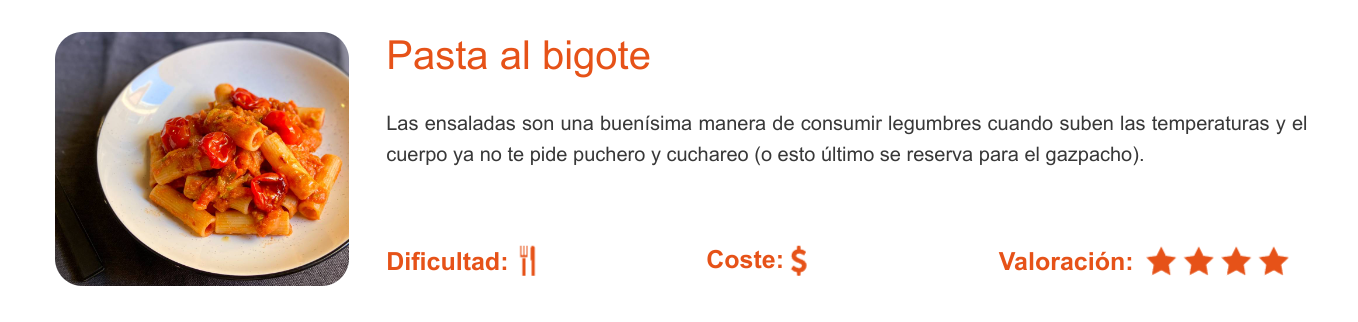
\includegraphics[frame,width=0.9\linewidth]{img/aic/receta.png}
    \vspace{-20pt}
\end{center}

Para cada uno de los resultados obtendremos los siguientes datos:

\begin{itemize}
    \item Nombre de la receta.
    \item Imagen principal de la receta.
    \item Pequeña introducción del texto introducido por el usuario.
    \item Dificultad.
    \item Coste.
    \item Valoración otorgada por los usuarios.
\end{itemize}

El título de la receta nos permitirá ir a la página principal de la receta para ver toda la información de la misma.

Al final de la página de búsqueda, dado que es posible que tengamos varias decenas de resultados, tendremos un sistema de paginación:

\begin{center}
    \vspace{-10pt}
    
\includegraphics[width=0.5\linewidth]{img/aic/paginado.png}
    \vspace{-20pt}
\end{center}

Haciendo uso de este sistema de paginación, podremos ir a los siguientes resultados y conocer cuántas páginas de resultados hemos obtenido tras introducir nuestros términos de búsqueda.

\section{Visualizar la información de la receta}

Al  hacer click sobre el título de cualquiera de las recetas que aparecen en los resultados de búsqueda iremos a la información completa de la receta. A la hora de visualizar la receta, la página resultante se puede dividir en distintas secciones.

La primera parte consta del nombre de la receta, junto con la dificultad, el coste, la valoración y los iconos para poder compartir la receta que será explicado posteriormente.


\begin{center}
    \vspace{-10pt}
    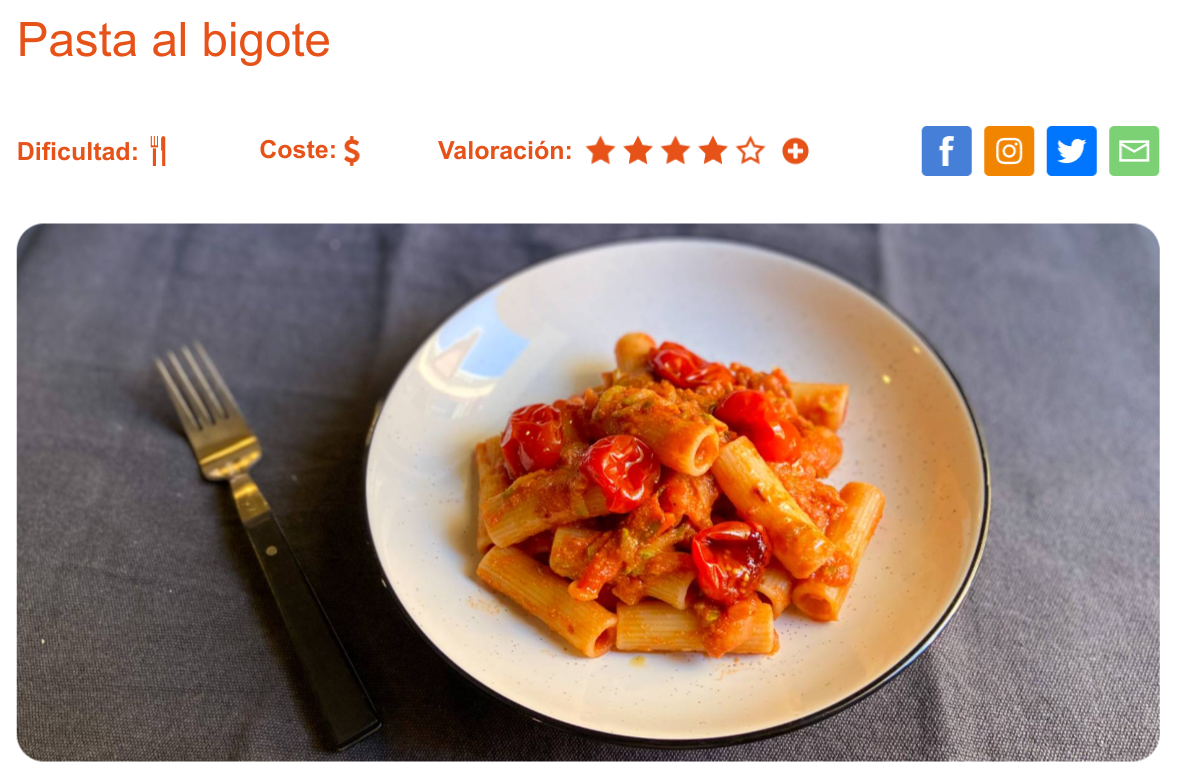
\includegraphics[width=0.7\linewidth]{img/aic/receta_1.png}
    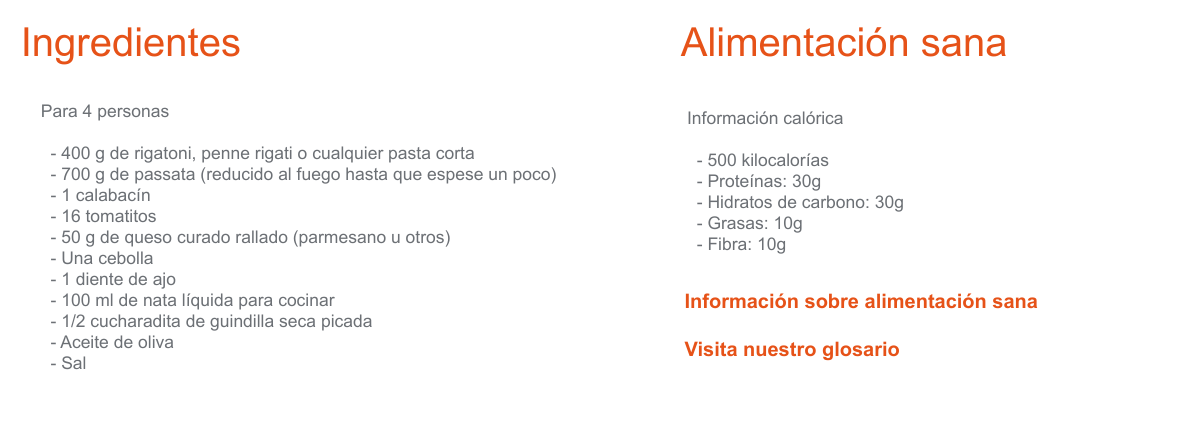
\includegraphics[width=0.7\linewidth]{img/aic/receta_2.png}
    \vspace{-20pt}
\end{center}

Debajo de la foto principal de la receta se puede distinguir dos apartados en forma de columnas, que son:

\begin{itemize}
    \item \textbf{Ingredientes}: Un desglose en forma de lista de los ingredientes necesarios para realizar la receta. En este caso se indica que es para cuatro personas.
    \item \textbf{Alimentación sana}: Información nutricional de la receta junto con dos enlaces a apartados creados sobre alimentación sana que serán explicados más adelante.
\end{itemize}

Tras esto, aparece el apartado de cómo se prepara la receta. Estos pasos son los introducidos por el usuario que ha registrado la receta.


\begin{center}
    \vspace{-10pt}
    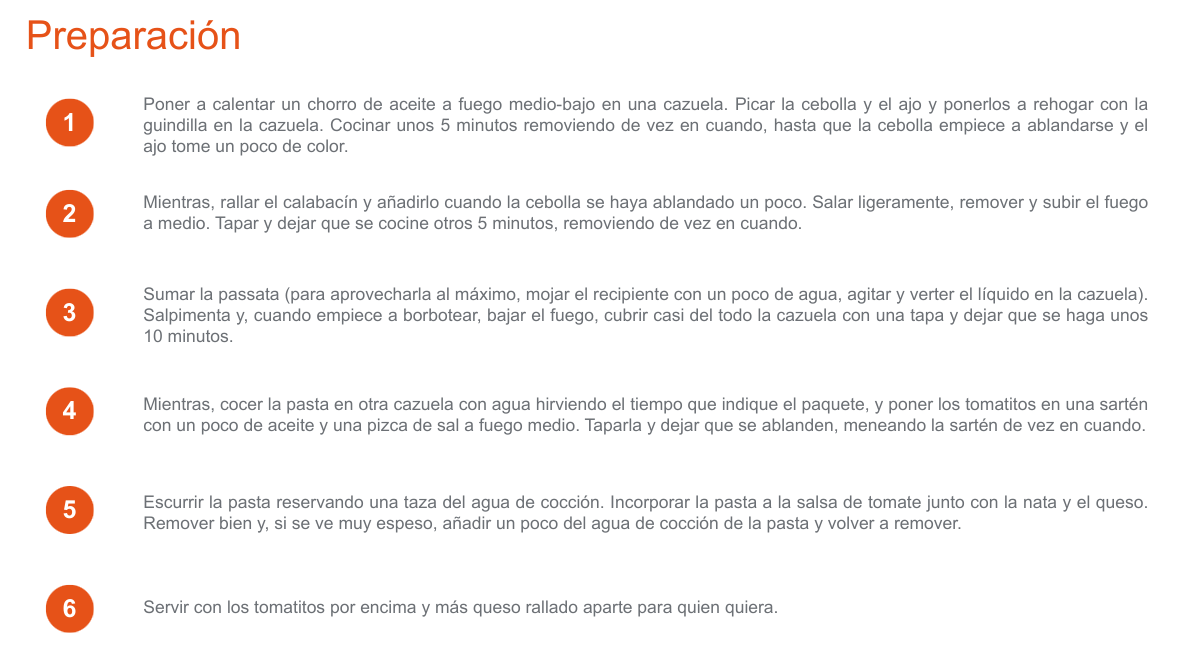
\includegraphics[width=0.7\linewidth]{img/aic/receta_3.png}
    
\includegraphics[width=0.7\linewidth]{img/aic/receta_4.png}
    \vspace{-20pt}
\end{center}

Y para finalizar, tal como se puede ver, aparece un apartado con los registros multimedia que el usuario haya podido incluir con la receta, como pueden ser vídeos o más imágenes.


\section{Compartir receta en redes sociales}

Junto con la información de la receta aparecen los iconos de varias redes sociales:

\begin{center}
    \vspace{-10pt}
    
\includegraphics[width=0.4\linewidth]{img/aic/compartir.png}
    \vspace{-20pt}
\end{center}

Al hacer click sobre cualquiera de estos iconos, se permitirá la compartición de la receta a través de las distintas redes sociales:

\begin{itemize}
    \item Facebook
    \item Instagram
    \item Twitter
    \item E-mail
\end{itemize}

Al hacer click en los iconos, nos aparecerá una pequeña ventana “\textit{pop-up}” para indicar con quién queremos compartir la receta:

\begin{center}
    \vspace{-10pt}
    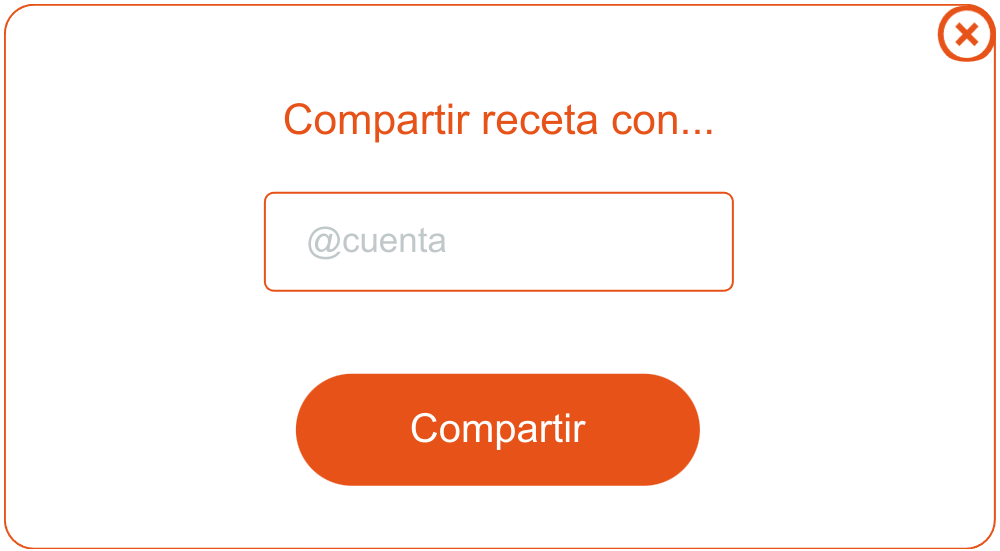
\includegraphics[width=0.4\linewidth]{img/aic/compartir_2.png}
    \vspace{-20pt}
\end{center}

Y tras darle al botón “compartir” se compartirá a través de la red social elegida o a través de un correo electrónico, de haber sido esa la opción elegida.


\section{Valorar receta}
En la visualización de la receta, entre el título y la foto principal, aparece la información de la valoración que tiene la receta actualmente junto con el símbolo “+”.

\begin{center}
    \vspace{-10pt}
    
\includegraphics[width=0.4\linewidth]{img/aic/valorar.png}
    \vspace{-20pt}
\end{center}

Este es el sistema utilizado para poder visualizar cuál es la valoración que los usuarios han otorgado a la receta. El símbolo “+” servirá a los usuarios para valorar la receta. Al hacer click sobre el símbolo se abrirá un \textit{pop-up} en el que podremos valorar la receta que estamos visualizando actualmente.

\begin{center}
    \vspace{-10pt}
    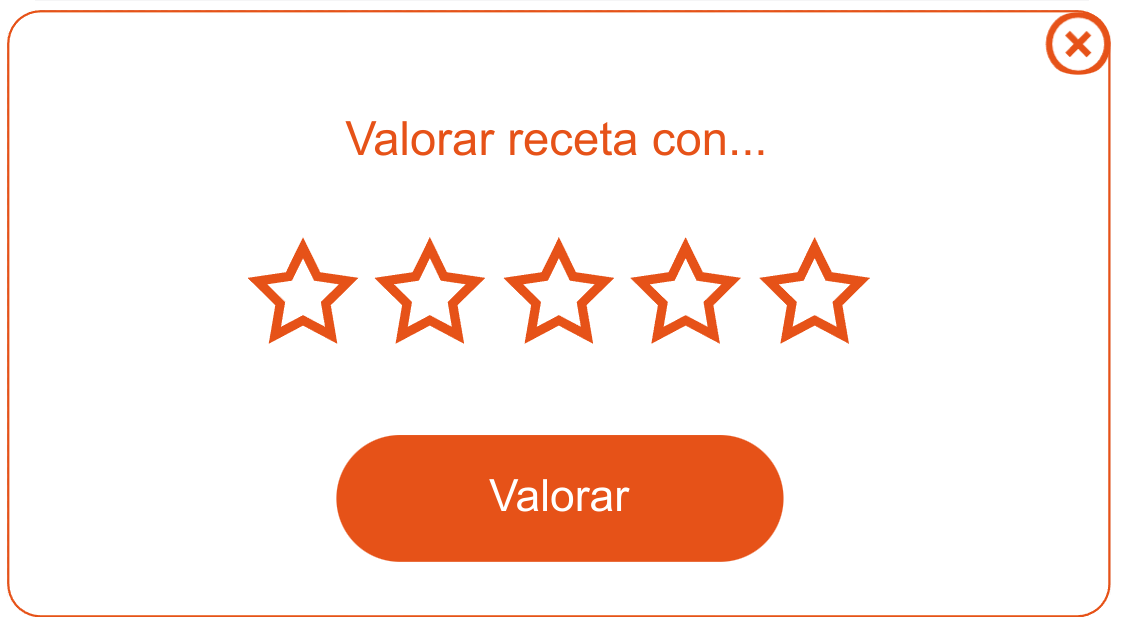
\includegraphics[width=0.4\linewidth]{img/aic/valorar_2.png}
    \vspace{-10pt}
\end{center}

De esta manera se podrá seleccionar el número de estrellas que el usuario quiere otorgar a la receta y después hacer click en el botón “valorar” para que dicha valoración se tenga en cuenta.


\chapter{Esquema de organización}

La nueva funcionalidad requerida por la \textbf{AIC} es el incorporar contenidos sobre alimentación sana a la aplicación web. Como se ha visto previamente, se ha decidido añadir la categoría “\textbf{Alimentación Sana}” al menú principal que encabeza la página web en todo momento.

Esta categoría es un desplegable que cuenta con tres apartados en las que se ha subdividido la información a modo de subcategorías:

\begin{center}
    \vspace{-10pt}
    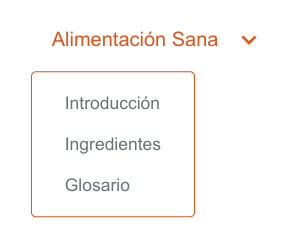
\includegraphics[width=0.4\linewidth]{img/aic/alimentacion_sana.png}
    \vspace{-20pt}
\end{center}


Cada una de estas opciones llevará al usuario a su página correspondiente que se detallarán a continuación.


\section{Introducción a la alimentación sana}
La finalidad de esta sección es la de dar información sobre la alimentación al usuario. Esta información ha sido tratada para que se use con un formato coloquial, pero que no por ello carezca de información científica y nutricional que será útil para el usuario.

Para no sólo dar información escrita, se ha hecho uso de la “\textbf{pirámide nutricional} en formato de imagen que permitirá al usuario hacer click en las distintas categorías que la forman para que pueda recibir más información de primera mano sobre la categoría seleccionada.

En la siguiente imagen se pueden ver las distintas secciones en las que se ha separado la pirámide y dónde se puede hacer click.
\begin{center}
    \vspace{-10pt}
    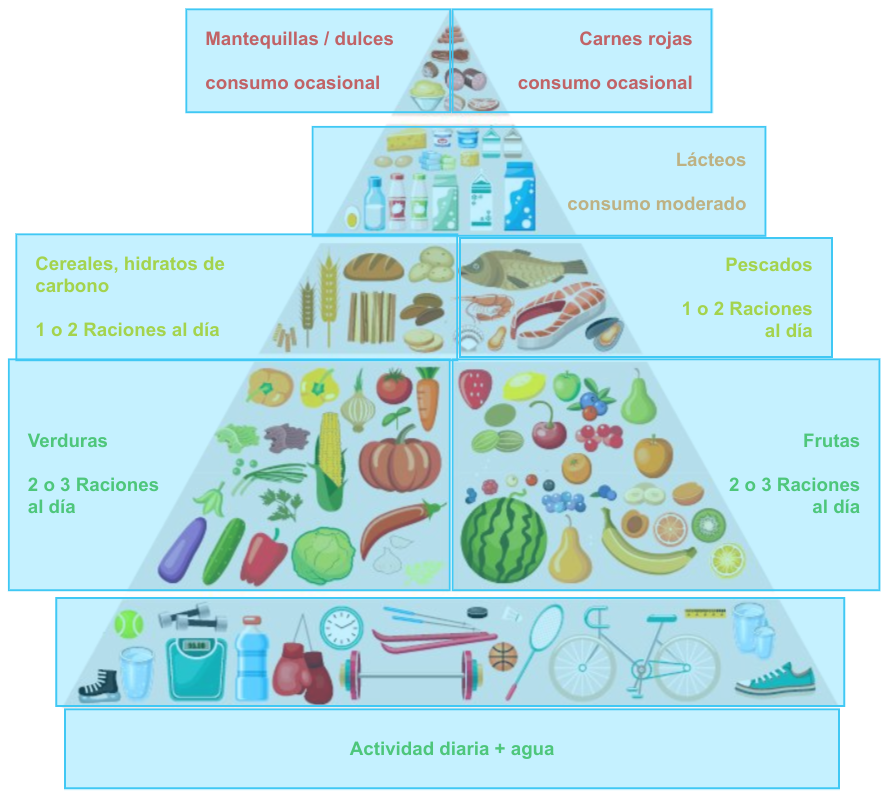
\includegraphics[width=0.6\linewidth]{img/aic/alimentacion_sana_piramide_click.png}
    \vspace{-20pt}
\end{center}

Tal como se puede apreciar en la imagen, existen distintas zonas en las que se puede hacer click, coincidiendo con los tipos de alimentos y la información, en formato coloquial, que es útil al usuario sobre el número de raciones diarias que debe de tomar.

Al hacer click sobre cualquiera de estas secciones le aparecerá un \textit{pop up} con más información, que aparece sobre la propia pirámide, y que podrá ampliar yendo al glosario.

\begin{center}
    \vspace{-10pt}
    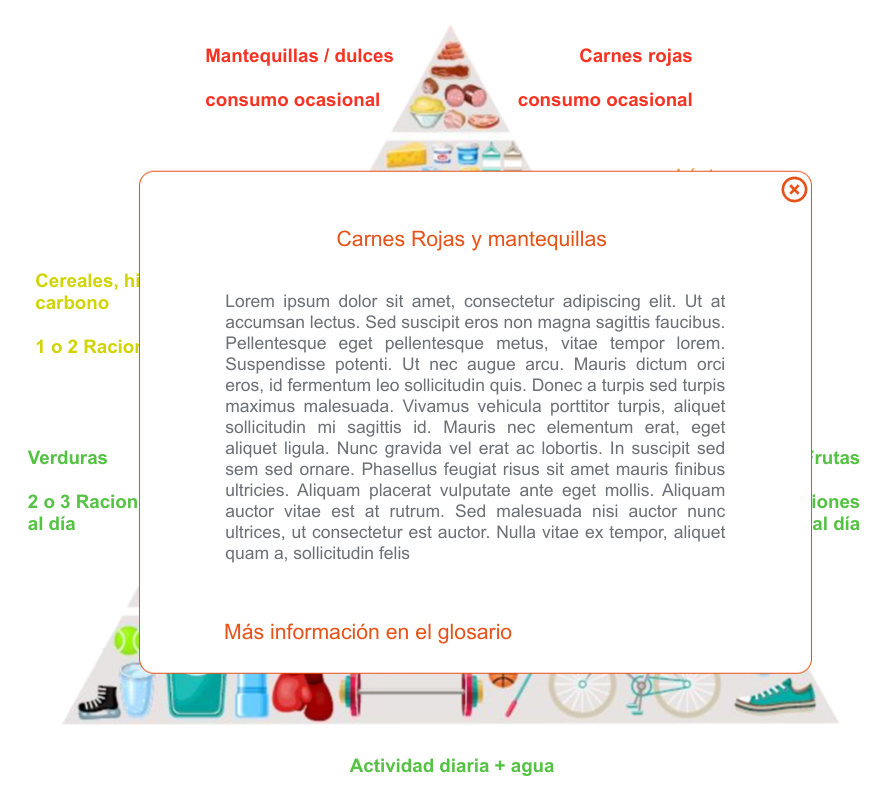
\includegraphics[width=0.6\linewidth]{img/aic/alimentacion_sana_piramide_click_2.png}
    \vspace{-20pt}
\end{center}

En este caso, la información trata sobre las carnes rojas, pero aparecerá la información requerida de la sección seleccionada.

Debajo de la pirámide se ha decidido añadir una tabla de manera en la que la información esté catalogada de manera más ordenada y dividida entre los distintos tipos de personas: bebe/infantil, joven/adolescente y adulto.

\begin{center}
    \vspace{-10pt}
    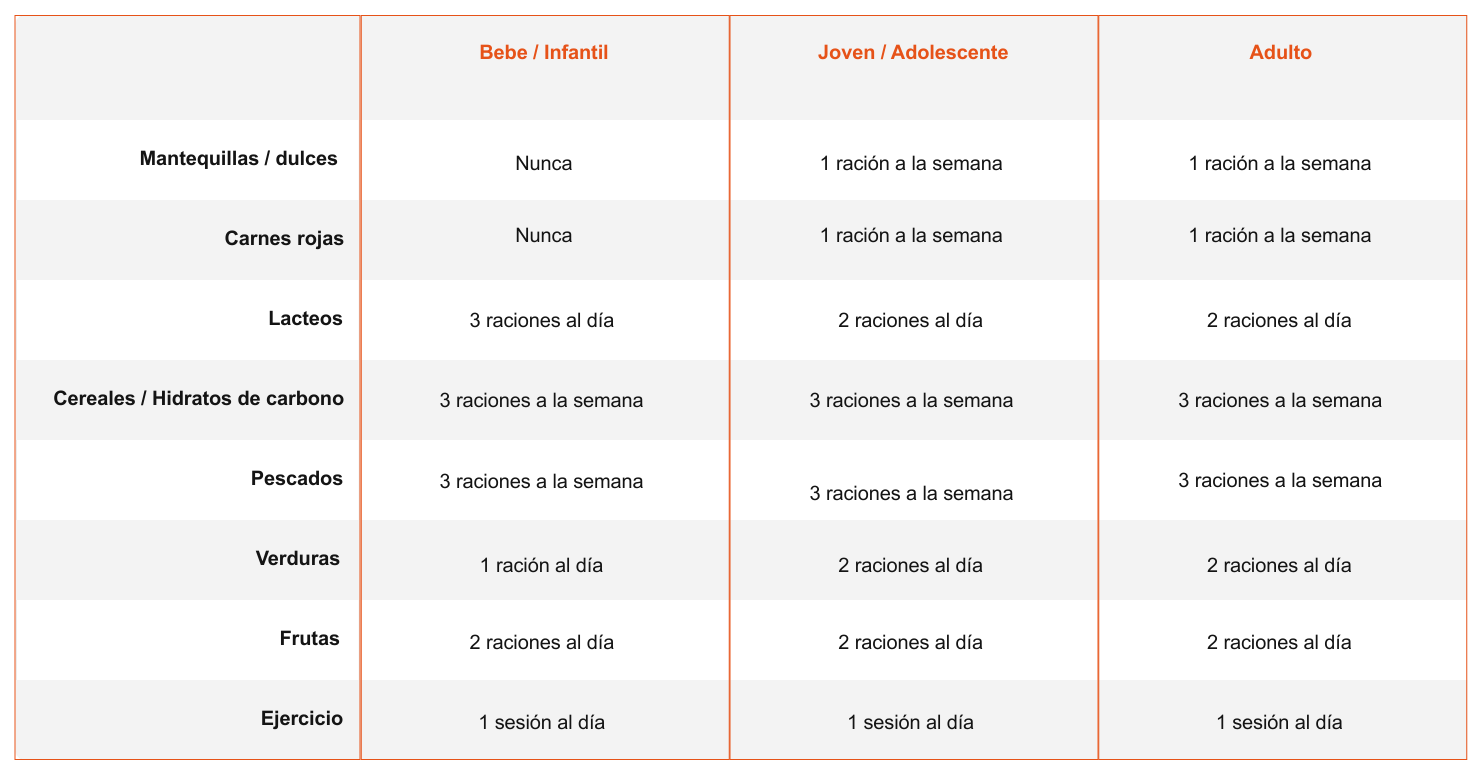
\includegraphics[width=0.9\linewidth]{img/aic/alimentacion_sana_tabla.png}
    \vspace{-20pt}
\end{center}

Haciendo uso de esta tabla, el usuario tendrá a su alcance la información categorizada de manera correcta.


\section{Ingredientes}
La segunda sección añadida en la categoría de alimentación sana es la referida a los \textbf{ingredientes}.

En esta página, para que la navegación sea sencilla a la hora de navegar entre todos los ingredientes existentes en la aplicación, se ha decidido añadir un menú de navegación indexado para poder acceder a los ingredientes teniendo en cuenta la primera letra del mismo:


\begin{center}
    \vspace{-10pt}
    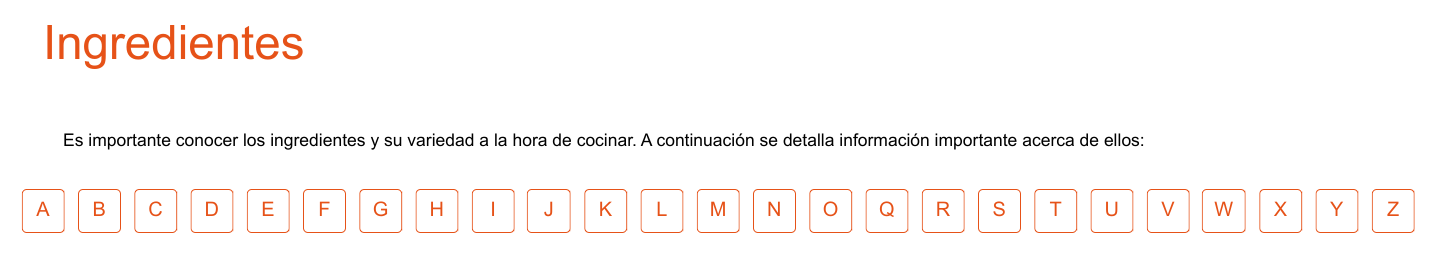
\includegraphics[frame,width=0.9\linewidth]{img/aic/ingredientes_indice.png}
    \vspace{-20pt}
\end{center}

De esta manera acceder al ingrediente buscado es más sencillo y más rápido para el usuario. Al llegar a la sección del ingrediente, se puede hacer click sobre el nombre que llevará al usuario a la página principal del ingrediente donde aparecerá más información del mismo:

\begin{center}
    \vspace{-10pt}
    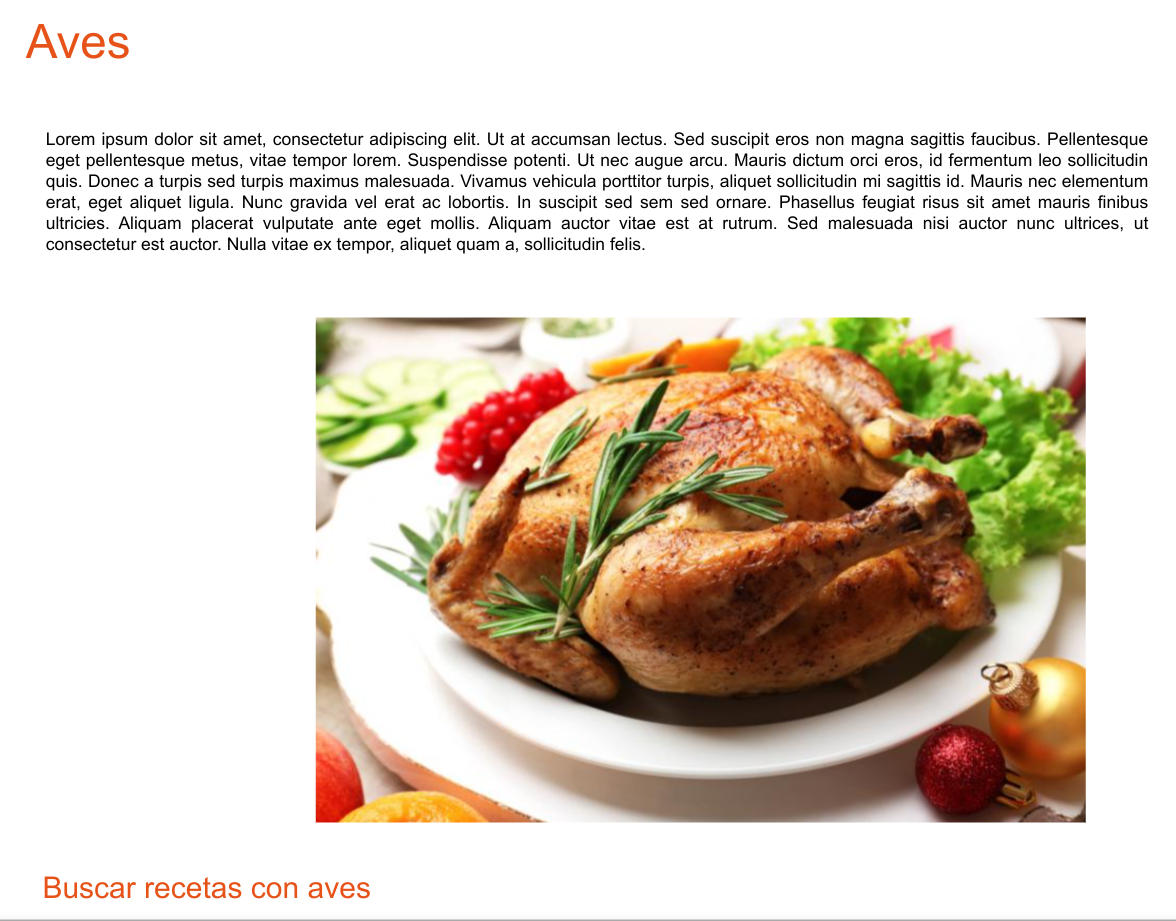
\includegraphics[frame,width=0.9\linewidth]{img/aic/ingredientes_info.png}
    \vspace{-20pt}
\end{center}

Viendo la imagen se puede observar, que para cualquier ingrediente, aparecerá información acerca del mismo junto con una imagen significativa de una receta. En la parte inferior de la página aparece un enlace con “\textbf{{\color{maincolor}Buscar recetas con...}}” que llevará al usuario a la página de búsqueda de recetas pero con el ingrediente ya seleccionado y mostrando sólo las recetas que al menos contengan dicho ingrediente.

Por último, cabe destacar que en la parte superior de la página aparecerá el “camino recorrido por el usuario” para que en todo momento sepa dónde se encuentra, y que cambiará dependiendo del ingrediente en el que se encuentre.

\begin{center}
    \vspace{-10pt}
    \textbf{{\color{maincolor}Alimentación sana > \space Ingredientes} >\space Aves}
    \vspace{-15pt}
\end{center}

Con todas estas opciones de categorización, junto con el camino del usuario, se trata de hacer que el tipo de navegación sea lo más sencillo en todo momento para el usuario.


\section{Glosario}
Para finalizar, la última subsección de la alimentación sana es el glosario, en el que se han añadido distintos términos junto con su información científica, pero de nuevo, usando lenguaje coloquial para los usuarios.

Al igual que sucede con los ingredientes, se ha añadido un índice para que la búsqueda de los términos resulte más sencilla.



\chapter{Mapa de navegación}
A la hora de navegar por la aplicación web de la \textbf{AIC} es importante que el usuario conozca en todo momento dónde se encuentra y cómo va a poder llegar a otros apartados a través de los enlaces.

Ya se ha comentado previamente que en todas las páginas se puede ver el “\textbf{camino recorrido por el usuario}”. Gracias a esto, el usuario podrá distinguir en qué sección, apartado o sub-apartado se encuentra y volver, de manera sencilla, sobre sus pasos.

A continuación se detalla un esquema de todas las navegaciones que el usuario puede realizar en toda la aplicación web:

\begin{center}
    \vspace{-10pt}
    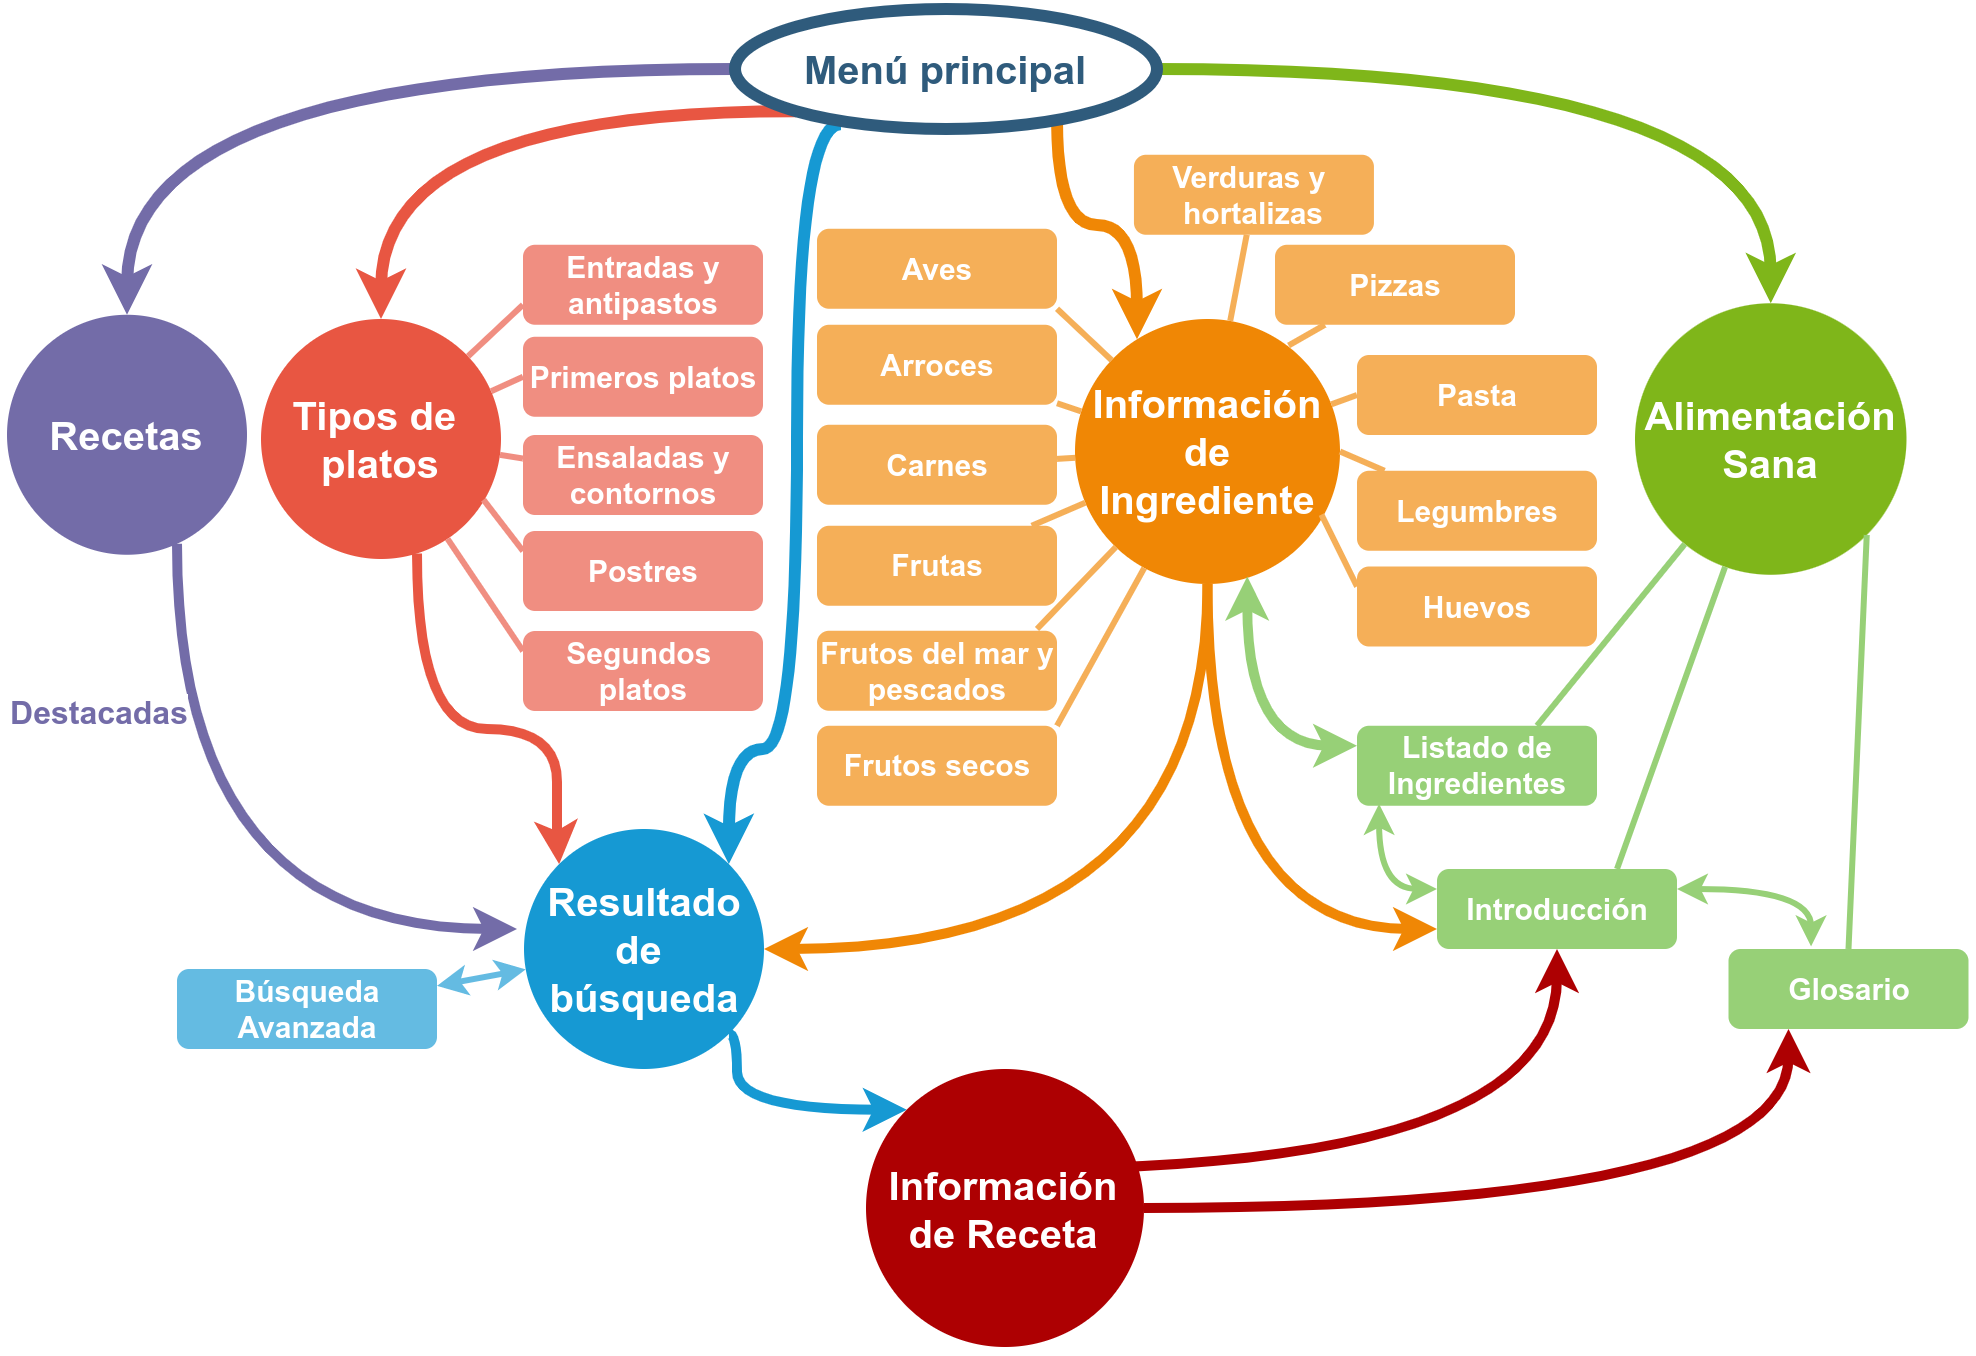
\includegraphics[width=0.9\linewidth]{img/mapa de navegacion.png}
    \vspace{-20pt}
\end{center}

El \hyperlink{menu_principal}{menú principal} es el origen desde el que se puede acceder a todas las secciones principales de la aplicación.

Como se puede ver, existe la posibilidad de navegar entre distintas secciones, como a continuación se va a detallar.



\section{Navegación en alimentación sana}

Desde la \textbf{AIC} se ha pedido la inclusión de información acerca de la alimentación sana, y ha sido, por tanto, necesario añadir navegación entre las propias secciones de la alimentación sana, así como con otras.

A continuación se puede ver el mapa de navegación que se ha realizado entre las subsecciones de alimentación sana que existe entre sí y con la información de los distintos ingredientes.

\begin{center}
    \vspace{-10pt}
    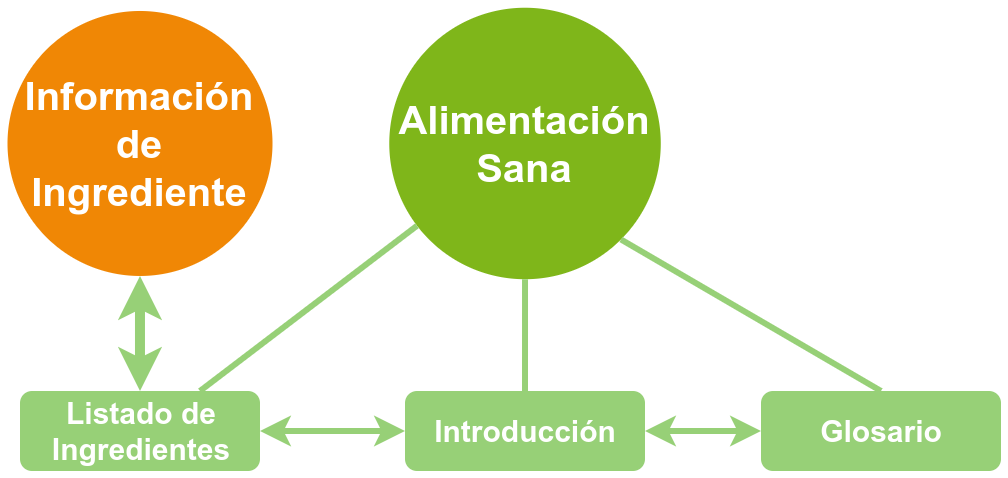
\includegraphics[width=0.5\linewidth]{img/mapa de navegacion2.png}
    \vspace{-20pt}
\end{center}

Observando la dirección de las flechas, se puede observar que la navegación es bidireccional en todo momento en las secciones de alimentación sana. De esta manera se pretende que el usuario tenga facilidad de buscar la información y volver a su punto de partida si así lo decide.

Recordar, tal como aparecería en el mapa de navegación completo, que a la información de alimentación sana también se puede llegar desde la información de la receta.


\chapter{Conclusiones}

Con todo lo dicho en este documento, se ha abordado la creación de un sistema a modo de prototipo general para la aplicación de la \textbf{AIC} buscando una alta fidelidad, y que el detalle y las funcionalidades mostradas sea lo más parecido a la realidad final de la aplicación. De esta manera, el cliente podrá saber cómo será el resultado final antes de realizar la programación.

También se ha puesto especial interés en el apartado de alimentación sana, ya que es una nueva funcionalidad y característica que es de gran interés para la \textbf{AIC} y quiere que los usuarios hagan uso de ella.

Con todo ello, el siguiente paso que queda es convertir el prototipo que podemos ver en la siguiente \href{https://yuki.github.io/VIU_03MASW/preview.html}{dirección web} y convertirlo en la aplicación web final para el cliente.


%\printbibliography[title={Referencias bibliográficas},heading=bibintoc]

\end{document}
